\documentclass[pdf]
{beamer}
\usepackage{tikz}
\usepackage{amssymb}
\usepackage{pgfplots}
\usepackage{listings}
\usetikzlibrary{fit,positioning,arrows,shapes.arrows,automata,calc,colorbrewer}
\tikzset{
  main/.style={circle, minimum size = 5mm, thick, draw =black!80, node distance = 10mm},
  connect/.style={-latex, thick},
  box/.style={rectangle, draw=black!100}
}
\mode<presentation>{}
%% preamble
\title{The Bootstrap Particle Filter}
\subtitle{... and how to implement it in Python}
\author{Paul Wilson}
\begin{document}

% Gauss distribution function.
\pgfmathdeclarefunction{gauss}{2}{%
  \pgfmathparse{1/(#2*sqrt(2*pi))*exp(-((x-#1)^2)/(2*#2^2))}%
}


%% title frame
\begin{frame}
\titlepage
\end{frame}

\begin{frame}{This talk}
\begin{itemize}
	\item Primarily: Understanding the bootstrap particle filter by implementing it in Python*
	\item Secondarily: Why the bootstrap filter is useful as a building block in other models.
\end{itemize}
\vspace{5mm}
\tiny * for a particular model
\end{frame}

\begin{frame}{Sequential Monte Carlo \& The Bootstrap Filter}
\begin{itemize}
	\item SMC methods are simulation-based methods for computing posterior distributions
	\item SMC can approximate $P(x_{0:t} | y_{0:t})$ for the model below.
	\item The bootstrap filter is a particular SMC algorithm with some nice properties.
\end{itemize}

\vspace{5mm}

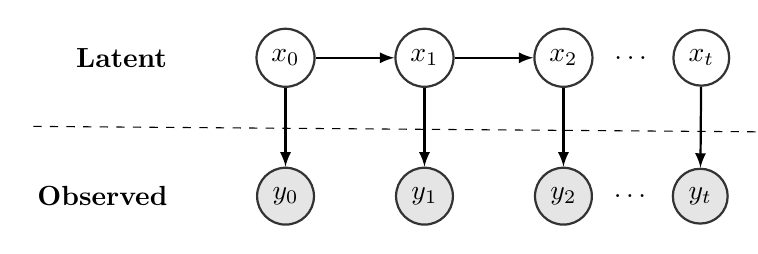
\begin{tikzpicture}
  \def\n{2}
  \node[box,draw=white!100] (Latent) {\textbf{Latent}};

  % Draw base case: x0, y0, and x0 -> y0
  \node[main] (x_0) [right=of Latent] {$x_0$};
  \node[main,fill=black!10] (y_0) [below=of x_0] {$y_0$};
  \path (x_0) edge [connect] (y_0);

  \foreach \i [evaluate = \i as \j using (\i - 1)] in {1,...,\n} {
  	% Draw next cases: x_t, y_t, x{t-1} -> x_t, and x_t -> y_t.l
    \node[main] (x_\i) [right=of x_\j] {$x_\i$};
    \node[main,fill=black!10] (y_\i) [below=of x_\i] {$y_\i$};
    \path (x_\j) edge [connect] (x_\i);
    \path (x_\i) edge [connect] (y_\i);
  }

  \node[box,draw=white!100,left=of y_0] (Observed) {\textbf{Observed}};

%  Final case: x_t, y_t, x_t -> y_t, and dashed line joining them.
  \node[main] (x_t) [right=of x_\n] {$x_t$};
  \node[main,fill=black!10] (y_t) [right=of y_\n] {$y_t$};
  \path (x_t) edge [connect] (y_t);
  \path (x_\n) -- node[auto=false]{\ldots} (x_t);
  \path (y_\n) -- node[auto=false]{\ldots} (y_t);

  % draw the dotted line connecting x_n -> x_t
  \draw [dashed, shorten >=-1cm, shorten <=-1cm]
      ($(Latent)!0.5!(Observed)$) coordinate (a) -- ($(x_t)!(a)!(y_t)$);
\end{tikzpicture}

\end{frame}


\begin{frame}{Example application: A bitcoin trading model}
\begin{itemize}
	\item We believe some traders are using `wash trading' to cause the bitcoin price to artificially rise.
	\item The market is either in `wash trade' state, or `normal' state.
	\item We want to identify when the market is in `wash trade' state so we can make a profit.
	\item Let's use $y_t \in \mathbb{R}$ to denote the change in price from $t - 1$ to $t$.
	\item When the market is in `wash trade' state, the average change will be some value $\mu > 0$.
	\item In `normal' market conditions, $y_t$ will remain around $0$.
\end{itemize}
\end{frame}


\begin{frame}{Example application: A bitcoin trading model}
\begin{figure}[htb]
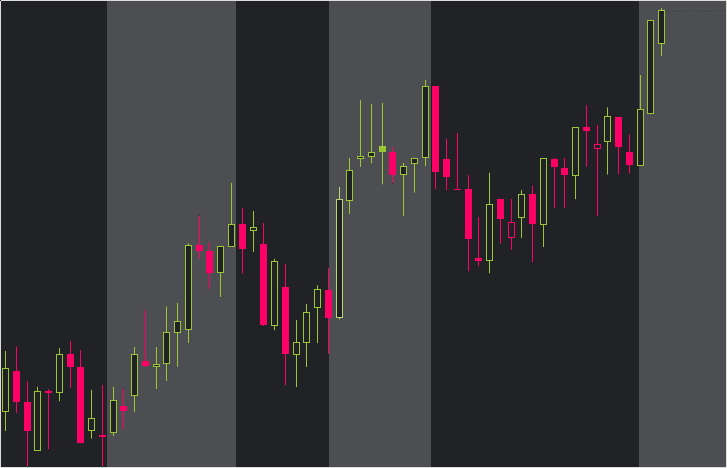
\includegraphics[width=\textwidth]{wash-trading.png}
\end{figure}
\tiny{Lighter regions might represent `wash trading' states}
\end{frame}

\begin{frame}{Distribution of price changes in `wash` and `non-wash` states.}

\begin{tikzpicture}
\def\n{2}
\begin{axis}[
  no markers, domain=-5:7, samples=100,
  axis y line*=left, ylabel=$P(y_t)$, ylabel near ticks, yticklabel pos=left,
  axis x line*=center, xlabel=$y_t$,
%  every axis y label/.style={at=(current axis.above origin),anchor=south},
  every axis x label/.style={at=(current axis.right of origin),anchor=west},
  height=5cm, width=12cm,
  xtick={0,1, \n}, ytick=\empty, xticklabels={0, $\frac{\mu}{2}$, $\mu$},
  enlargelimits=false, clip=false, axis on top,
  grid = major
  ]
 
  \addplot [fill=cyan!20, draw=none, domain=-5:1] {gauss(\n,1)} \closedcycle;
  \addplot [fill=cyan!20, draw=none, domain=1:7] {gauss(0,1)} \closedcycle;
  \addplot [very thick,cyan!50!black] {gauss(0,1)};
  \addplot [very thick,cyan!50!black] {gauss(\n,1)};

\end{axis}
\end{tikzpicture}

A simple model is to decide for `wash trade` state when an observation $y_i > \frac{\mu}{2}$.

However, we want to incorporate time-series information to make better predictions.

We'll make the assumption that if the market is in `wash trade' or `non-wash-trade' state, it's likely to stay there with probability $p$.

\end{frame}


\begin{frame}{The `sticky-state' hidden markov model}
Latent states $x_i \in \{0, 1\}$ generate observations $y_i \in \mathbb{R}$ from
a normal distribution with mean $\mu x_i$ and variance $1$.

\vspace{5mm}

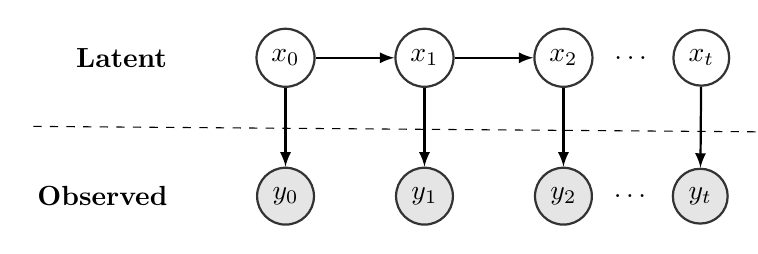
\begin{tikzpicture}
  \def\n{2}
  \node[box,draw=white!100] (Latent) {\textbf{Latent}};

  % Draw base case: x0, y0, and x0 -> y0
  \node[main] (x_0) [right=of Latent] {$x_0$};
  \node[main,fill=black!10] (y_0) [below=of x_0] {$y_0$};
  \path (x_0) edge [connect] (y_0);

  \foreach \i [evaluate = \i as \j using (\i - 1)] in {1,...,\n} {
  	% Draw next cases: x_t, y_t, x{t-1} -> x_t, and x_t -> y_t.
    \node[main] (x_\i) [right=of x_\j] {$x_\i$};
    \node[main,fill=black!10] (y_\i) [below=of x_\i] {$y_\i$};
    \path (x_\j) edge [connect] (x_\i);
    \path (x_\i) edge [connect] (y_\i);
  }

  \node[box,draw=white!100,left=of y_0] (Observed) {\textbf{Observed}};

%  Final case: x_t, y_t, x_t -> y_t, and dashed line joining them.
  \node[main] (x_t) [right=of x_\n] {$x_t$};
  \node[main,fill=black!10] (y_t) [right=of y_\n] {$y_t$};
  \path (x_t) edge [connect] (y_t);
  \path (x_\n) -- node[auto=false]{\ldots} (x_t);
  \path (y_\n) -- node[auto=false]{\ldots} (y_t);

  % draw the dotted line connecting x_n -> x_t
  \draw [dashed, shorten >=-1cm, shorten <=-1cm]
      ($(Latent)!0.5!(Observed)$) coordinate (a) -- ($(x_t)!(a)!(y_t)$);
\end{tikzpicture}

\vspace{5mm}

The transition density $ p(x_i | x_{i - 1})$ means the system likes to `stick`
in the current state with probability $p$.

\[   
p(x_i | x_{i - 1}) = 
     \begin{cases}
       \text{$p$,} &\quad\text{if  } x_i = x_{i - 1} \\
       \text{$1 - p$,} &\quad\text{otherwise.} \\ 
     \end{cases}
\]

Finally, assume $ X_0 \sim Bernoulli(\frac{1}{2}) $

\end{frame}




%%%%% Generating data with Python %%%%%
\begin{frame}[fragile]{Generating Data with Python (part 1)}
  This code specifies the model dynamics. It'll come in handy later to plug in to the bootstrap filter.

  \begin{figure}
  \centering
      \tiny
   \lstset{language=python,
		basicstyle=\ttfamily,
		keywordstyle=\color{blue}\ttfamily,
		stringstyle=\color{red}\ttfamily,
		commentstyle=\color{green}\ttfamily,
		morecomment=[l][\color{magenta}]{\#}
   }
         \lstinputlisting{code-fragments/simulate_setup.py}
   \end{figure}

\end{frame}

\begin{frame}[fragile]{Generating Data with Python (part 2)}
  We can use the previous code to generate sequences of states and observations from the model.
  
  \begin{figure}
  \centering
      \tiny
   \lstset{language=python,
		basicstyle=\ttfamily,
		keywordstyle=\color{blue}\ttfamily,
		stringstyle=\color{red}\ttfamily,
		commentstyle=\color{green}\ttfamily,
		morecomment=[l][\color{magenta}]{\#}
   }
         \lstinputlisting{code-fragments/simulate_forward.py}
   \end{figure}
\end{frame}





\begin{frame}{The Bootstrap Particle Filter}
The idea:

\begin{itemize}
  \item Maintain a list of $N$ particles
  \item Each particle is a trajectory of states $\mathbf{x}^{(i)}_{0:t}$.
  \item Simulate each particle one step forward
  \item Weight each particle by the likelihood of the observed data, $P(y_{t+1} | x^{(i)}_{t+1})$
  \item Resample the list of particles according to their weights.
\end{itemize}
\end{frame}



\begin{frame}{The Bootstrap Particle Filter: Simulate forward}
	\begin{itemize}
		\item "Simulating forward" means generating $x_t \sim p(x_t | x_{t - 1})$
	    \item This diagram shows a single trajectory (particle), with time moving left to right.
    \end{itemize}
	
	\vspace{5mm}
	
	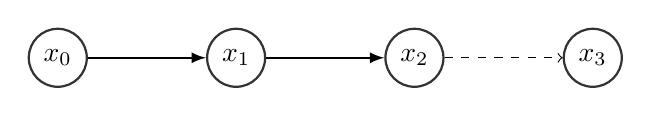
\begin{tikzpicture}
		\def\T{2}
		\node[main] (x_{0}) {$x_0$};
		\foreach \t [evaluate = \t as \u using (int(\t - 1))] in {1,...,\T} {
		  \node[main] (x_{\t}) [right=1.5cm of x_{\u}] {$x_{\t}$};
		  \path (x_{\u}) edge [connect] (x_{\t});
		}
		\node[main] (x_{3}) [right=1.5cm of x_{\T}] {$x_3$};
		\draw[dashed, ->] (x_{\T}) -- (x_{3});
	\end{tikzpicture}

\end{frame}



\begin{frame}{The Bootstrap Particle Filter: Weight particles}
	\begin{itemize}
		\item The weight of each trajectory is the likelihood for $y_t$ given the current state.
		\item Weights are normalised before the resampling step
	\end{itemize}
	
	\vspace{5mm}
	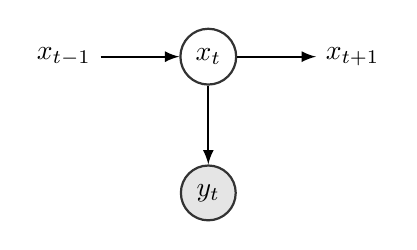
\begin{tikzpicture}
	  	\node (prev) {$x_{t-1}$};
	  	\node[main] (cur) [right=of prev] {$x_{t}$};
	  	\node (next) [right=of cur] {$x_{t+1}$};
	  	
	  	\node[main,fill=black!10] (obs) [below=of cur] {$y_t$};
	  	
    	\path (prev) edge [connect] (cur);
    	\path (cur) edge [connect] (next);
    	\path (cur) edge [connect] (obs);
	\end{tikzpicture}
\end{frame}



\begin{frame}{The Bootstrap Particle Filter: Resampling}
	\begin{itemize}
		\item Three trajectories are shown, with time moving downwards
		\item Colours denote particle ancestry
		\item After resampling, the first particle has been propagated twice.
	\end{itemize}

	\resizebox{10.0cm}{!}{%
	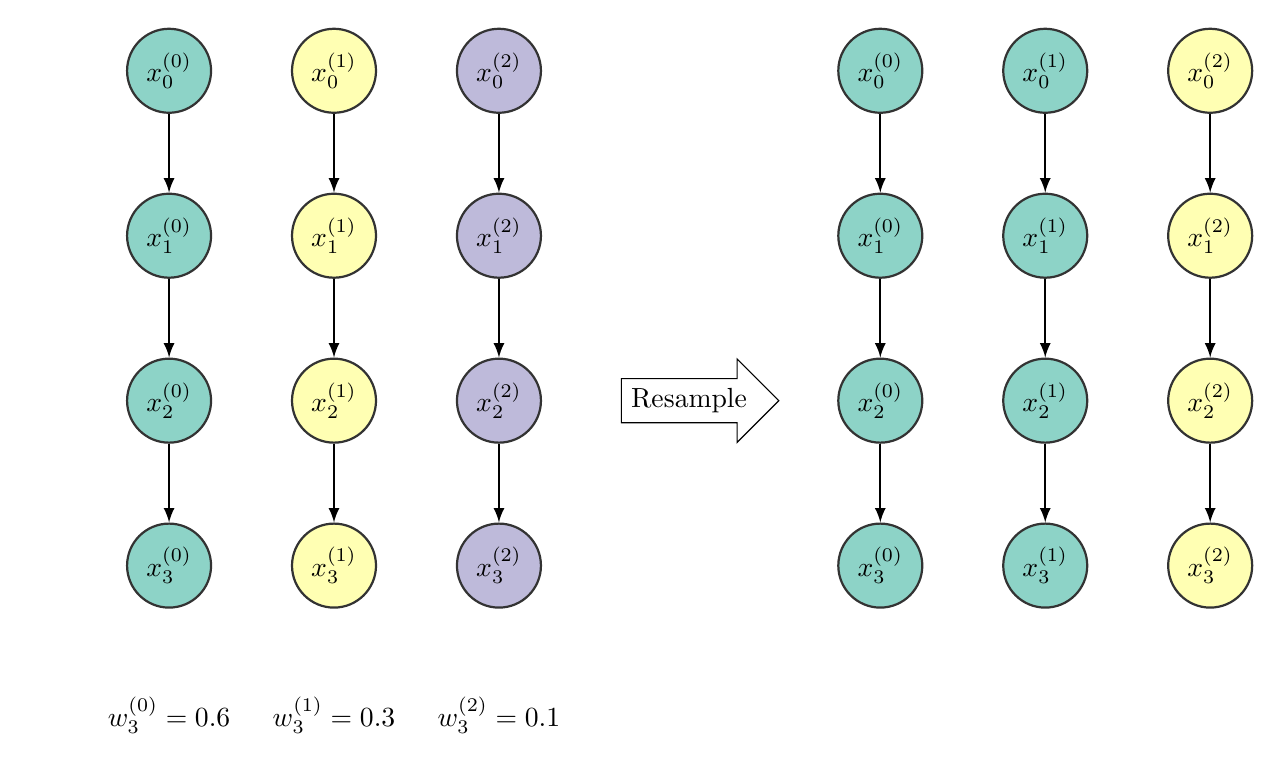
\begin{tikzpicture}
	  \def\N{2}
	  \def\T{3}

	  % Lattice #1
	  % Invisible dummy node.
	  \node[box,draw=white!100] (x^{-1}_{0}) {};

	%  \foreach \n [evaluate = \n as \m using (int(\n - 1))] in {0,...,\N} {
	  \foreach \n/\c [evaluate = \n as \m using (int(\n - 1))] in {0/Set3-A, 1/Set3-B, 2/Set3-C} {
		\node[main, fill=\c] (x^{\n}_{0}) [right=of x^{\m}_{0}] {$x^{(\n)}_0$};
		
		\foreach \t [evaluate = \t as \u using (int(\t - 1))] in {1,...,\T} {
		  \node[main, fill=\c] (x^{\n}_{\t}) [below=of x^{\n}_{\u}] {$x^{(\n)}_{\t}$};
		  \path (x^{\n}_{\u}) edge [connect] (x^{\n}_{\t});
		}
	  }

	  % Weights
	  \node (w_0) [below=of x^{0}_{\T}] {$w_3^{(0)} = 0.6$};
	  \node (w_1) [below=of x^{1}_{\T}] {$w_3^{(1)} = 0.3$};
	  \node (w_2) [below=of x^{2}_{\T}] {$w_3^{(2)} = 0.1$};

	  % "Resample" arrow.
	  \node[draw, single arrow] (arrow) [right=of x^{\N}_{2}] {Resample};


	  % Lattice #2
	  \node[box,draw=white!100] (x2^{-1}_{0}) [right=2.5cm of x^{\N}_{0}] {};

	  \foreach \n/\c [evaluate = \n as \m using (int(\n - 1))] in {0/Set3-A, 1/Set3-A, 2/Set3-B} {
		\node[main, fill=\c] (x2^{\n}_{0}) [right=of x2^{\m}_{0}] {$x^{(\n)}_0$};
		
		\foreach \t [evaluate = \t as \u using (int(\t - 1))] in {1,...,\T} {
		  \node[main, fill=\c] (x2^{\n}_{\t}) [below=of x2^{\n}_{\u}] {$x^{(\n)}_{\t}$};
		  \path (x2^{\n}_{\u}) edge [connect] (x2^{\n}_{\t});
		}
	  }

	\end{tikzpicture}%
	}%

\end{frame}

\begin{frame}{The Bootstrap Particle Filter: Pseudocode}
\fbox{\parbox{\textwidth}{The Bootstrap Filter
	\begin{enumerate}
		\item \underline{\textit{Initialization}},
			  $t = 0$.
		\begin{itemize}
			\item For $i = 1, ..., N$, sample $\mathbf{x}^{(i)}_0 \sim p(\mathbf{x}_0)$ and set $t = 1$.
		\end{itemize}
	
		\item \underline{\textit{Importance sampling step}}
		\begin{itemize}
			\item For $i = 1, ..., N$, sample
			$\tilde{\mathbf{x}}^{(i)}_t \sim p(\mathbf{x}_t | \mathbf{x}_{t-1}^{(i)})$ 
    	    and set $\tilde{\mathbf{x}}^{(i)}_{0:t} = 
    	    (\mathbf{x}_{0:t - 1}^{(i)}, \tilde{\mathbf{x}}_t^{(i)})$
    	    
    	    \item For $i = 1,..,N$, evaluate the importance weights
         	$$ \tilde{w}^{(i)}_t = p(\mathbf{y}_t | \tilde{\mathbf{x}}_t^{(i)}) $$
         	
         	\item Normalise the importance weights
         	
		\end{itemize}
		
		\item \underline{\textit{Selection Step}}
		\begin{itemize}
			\item Resample with replacement $N$ particles
			$\big(\mathbf{x}_{0:t}^{(i)}; i = 1,...,N\big)$
			from the set
			$\big(\tilde{\mathbf{x}}_{0:t}^{(i)}; i = 1,...,N\big)$
			according to the importance weights.
			
			\item Set $t \gets t + 1$ and go to step 2.
		\end{itemize}
		
	\end{enumerate}
}}

\tiny{
An introduction to Sequential Monte Carlo Methods, (Doucet, de Freitas, Gordon, p 11)
}

\end{frame}

\begin{frame}[fragile]{The Bootstrap Particle Filter: Python implementation}
  \begin{figure}
  \centering
      \tiny
   \lstset{language=python,
		basicstyle=\ttfamily,
		keywordstyle=\color{blue}\ttfamily,
		stringstyle=\color{red}\ttfamily,
		commentstyle=\color{green}\ttfamily,
		morecomment=[l][\color{magenta}]{\#}
   }
         \lstinputlisting{code-fragments/bootstrap.py}
   \end{figure}
\end{frame}


\begin{frame}{Discussion}
	\begin{itemize}
		\item The bootstrap filter doesn't need to `hard-code' model dynamics
		\item in the previous Python code you could easily factor out model-specific code.
		\item PMCMC methods exploit this, so inference can be made for arbitrary models with
			  \textit{``limited design effort on the users' part.''}
		\item PMCMC can be useld, for example, to infer distributions over parameters $\mu$ and $p$ in our
			  example model.
%		\item Imagine, for example, a system whose observations are from a Gaussian at odd-numbered times,
%			  and from a Poisson at even-numbered times.
	\end{itemize}
\end{frame}



\begin{frame}{Experiments!}

Three models are compared on simulated data of $40$ observations.

\begin{itemize}
	\item The Bootstrap particle filter implemented above
	\item The Viterbi algorithm
	\item The `Baseline' model - deciding for state $x_i = 1 \text{if } y_i > \frac{\mu}{2}$.
\end{itemize}

I measured accuracy as the percentage of states $x_i$ correctly guessed, averaged over $10,000$ runs for the parameters $ p = 0.95 $, $\mu = 1$, and $N = 1000$ particles.

\vspace{5mm}

\begin{table}
	\centering
	\begin{tabular}{ l | c }
	  algorithm & accuracy \\
	  \hline
	  Baseline 	& 69\% \\
	  Viterbi 	& 86\% \\
	  Bootstrap & 87\% \\
	\end{tabular}
\end{table}

\end{frame}

\begin{frame}{Experiments Discussion}
\begin{itemize}
	\item Minor difference between Viterbi and Bootstrap might be due to metric chosen.*
	\item Viterbi returns the MAP estimate of the whole sequence, not each state individually.
	\item Baseline result is equal to $f(x = 0.5 | \mu = 1, \sigma^2 = 1)$ where $f$ denotes the normal CDF.
\end{itemize}
\tiny * or a bug
\end{frame}

%\begin{frame}{More Experiments!}
%Heatmap over grid of $p \in [0.5, 1]$ and $\mu \in [0, 3]$.
%Expected outcome: incorporating time series information only matters when $\mu$ is small and $p$ is large.

%If $\mu$ is large, then there is little overlap between the two distributions.

%If $p$ is close to $0.5$, then each observation is more-or-less independent.
%\end{frame}


\end{document}